\documentclass{beamer}
\usepackage{libs/beamerthemeIFS} % usando tema personalizado. 
\usepackage{libs/formatacaoCSharp} % usando formatação de código C#

\usepackage{pgfpages}
% \setbeameroption{show notes}
% \setbeameroption{show notes on second screen=right}
\author{Prof. Fulano de Tal \\	\url{meu@email.dominio.br}}
\date{\today}

%%%%%%%%%%%%%%%%%%%%%%%%%%%%%%%%%%%%%%%%%%%%
\title{Programação Web 2}
\subtitle{Aula 02 - A linguagem \CS}
%%%%%%%%%%%%%%%%%%%%%%%%%%%%%%%%%%%%%%%%%%%%

\begin{document}

\begin{frame}[t]
	\maketitle
\end{frame}

% Descomente as linhas abaixo se desejar colocar um sumário de todas as seções
\begin{frame}[t]{Sumário}
\tableofcontents
\end{frame}


\def\sectionname{}
\def\insertsectionnumber{}
\def\subsectionname{}
\def\insertsubsectionnumber{}
%
\AtBeginSection{\frame{\sectionpage}\addtocounter{framenumber}{-1}}
%
%
%\AtBeginSubsection{\frame{\subsectionpage}\addtocounter{framenumber}{-1} }
%\AtBeginSubsubsection{\frame{\subsubsectionpage}\addtocounter{framenumber}{-1} }




%%%%%%%%%%%%%%%%%%%%%%%%%%%%%%%%%%%%%%%%%%%%
% Inicio do documento
%%%%%%%%%%%%%%%%%%%%%%%%%%%%%%%%%%%%%%%%%%%%




%\section{Introdução}
\section{Conceitos básicas}


\begin{frame}
\frametitle{Introdução ao \CS}
\begin{outline}
	\1 Regras Gerais
	\2 As instruções devem estar dentro de um escopo e sempre ser finalizadas com um ponto e vírgula;
	\2 \CS é \textit{case-sensitive};
	\2 \CS é uma linguagem fortemente tipada, ou seja, todas as variáveis e objetos devem ter um tipo declarado;
	\2 Os tipos podem ser divididos em:
	\3 \textbf{\textit{Value Types}}: possuem o valor da variável.
	\3 \textit{\textbf{Reference Types}}: possuem uma referência para posição de memória onde o valor está alocado.
	\2 As variáveis armazenam informações na memória e segue a convenção de nomes da linguagem Java.
	
\end{outline}
\end{frame}

\subsection{Identificadores}
\begin{frame}[fragile]
\frametitle{Identificadores}
\begin{outline}
	\1 São nomes arbitrários para variáveis, métodos, tipos definidos pelo usuários, etc...
	\1 Devem ser compostos por caracteres Unicode;
	\1 É \textit{case sensitive} e \textit{locale-independente}
\end{outline}
\begin{lstlisting}
<Tipo> Nome, nome;
<Tipo> idade, Idade;
\end{lstlisting}
\end{frame}


\subsection{Variáveis}

\begin{frame}[fragile]
\frametitle{Variáveis}
\begin{outline}
	\1 Armazenam informações na memória e segue a convenção de nomes da linguagem Java.
	\2 [Ex.:] \begin{lstlisting}
	string nome;
	int idade = 50;
	\end{lstlisting}
	\1 O tipo pode ser definido de forma implícita através do modificador var
	\2 [Ex.:] \begin{lstlisting}
	var i = 5;
	var str = "Olá Mundo";
	\end{lstlisting}
	
\end{outline}
\end{frame}


\subsection{Constantes}

\begin{frame}[fragile]
\frametitle{Constantes}
\begin{outline}
	\1 Valores imutáveis que não podem ser alterados durante a execução do programa.
	\1 [Ex.:] \begin{lstlisting}
public const int MESES = 12;	
	\end{lstlisting}
\end{outline}

\end{frame}

\subsection{Propriedades}

\begin{frame}
\frametitle{Propriedades}
\begin{outline}
\1 Uma propriedade é um membro que fornece um mecanismo flexível para ler, escrever ou calcular o valor de um campo privado.
\1 As propriedades podem ser usadas como se fossem membros de dados públicos, mas eles são realmente métodos especiais chamados acessadores.
\1 Isso permite que os dados sejam acessados facilmente e ainda ajuda a promover a segurança e a flexibilidade dos métodos.
\1 As propriedades permitem que uma classe exponha, de maneira pública, a forma de obter e definir valores e ocultar a implementação ou o código de verificação.
\1 As propriedades podem ser:
	\2 lidas e gravadas (elas possuem um acessador \textit{get} e outro \textit{set});
	\2 somente leitura (elas possuem um acessador de acesso, mas nenhum \textit{set});
	\2 somente de gravação (só tem um accessor \textit{set} definido).
\end{outline}
\end{frame}


\begin{frame}[fragile]
\frametitle{Exemplo de propriedade}
\begin{lstlisting}
using System;

class TimePeriod
{
	public double Segundos
	{
		get ;
		private set ;
	}
}
\end{lstlisting}
\end{frame}

\begin{frame}[fragile]
\frametitle{Exemplo de propriedade}
\begin{lstlisting}
using System;

class TimePeriod
{
	private double segundos;	
	public double Segundos
	{
		get { return segundos; }
		protected set { this.segundos = value;} 
	}
}
\end{lstlisting}
\end{frame}


\begin{frame}[fragile]
\frametitle{Exemplo de propriedade}
\begin{lstlisting}
using System;

class TimePeriod
{
	private double seconds;	
	public double Hours
	{
		get { return seconds / 3600; }
		set { 
			if (value < 0 || value > 24)
			throw new ArgumentOutOfRangeException(
			$"{nameof(value)} must be between 0 and 24.");
			
			seconds = value * 3600; 
		}
	}
}
\end{lstlisting}
\end{frame}



\subsection{Namespaces}

\begin{frame}
\frametitle{Namespaces}
\begin{outline}
	\1 Organizam o código de grandes projetos;
	\1 São delimitados através do uso do operador ponto;
	\1 A diretiva using evita a necessidade de especificar o nome do \textit{namespace} para cada classe;
	\1 O \textit{namespace} global é o \textit{namespace} "raíz": \codef{global::System} sempre irá se referir ao \textit{namespace} System do .NET Framework;
	\1 É uma organização lógica!
\end{outline}
\begin{block}{Package vs Namespace}
No Java o \codef{Package} impõe uma organização física (além da lógica). Já no \CS o \codef{namespace} só há organização lógica!
\end{block}
\end{frame}


\begin{frame}
\frametitle{Namespace}
\begin{outline}
	\1 [] {\LARGE Atenção}
	\1 [] A documentação do .NET Framework recomendam o seguinte critério para nomear os espaços de nomes:
	\2 [] {<Empresa>.(<Produto>|<Tecnologia>) }
	\2 [] \qquad [.<Caracteristica>][.<Subnamespace>]
	
\end{outline}



\end{frame}

\subsection{Tipos}
\begin{frame}
\frametitle{Tipos}
\begin{outline}
	\1 Descrevem valores e especificam as convenções que todos os valores daquele tipo devem suportar.
	\1 Podem ser:
	\2 \textit{Value types} (Valores): tipos internos e predefinidos como inteiros e de ponto flutuante;
		\3 É possível criar um tipo que também aceita o valor nulo (\textit{Nullable Types})
		\3 um \textit{nullable type} pode representar o valor correto (dentro da faixa especificada para o tipo) com o valor adicional NULL.
	\2 \textit{Reference types} (Objetos): tipos que se autodescrevem (objetos), ponteiros e interfaces;
	\1 \textbf{Atenção:} duas entidades são do mesmo tipo se possuírem representação e comportamento compatível entre si.

\end{outline}
\note{Autodescrevem: que sua definição contém (a) a representação assumida por todos os valores daquele tipo; (b) as operações podem ser realizadas com os valores daquele tipo e (c) o código que implementa tanto a representação quanto o comportamento é definido.}	
\end{frame}

\subsubsection{Tipos predefinidos}
\begin{frame}
\frametitle{Tipos predefinidos}
\begin{table}[]
	\centering
	\label{my-label}
	\begin{tabular}{|l|l|l|}
		\hline
		\textbf{Tipo}~\footnotemark & \textbf{Alias}\footnotemark  & \textbf{Descrição}                     \\ \hline
		Boolean         & bool              &                                        \\ \hline
		Char            & char              &                                        \\ \hline
		Object          & object            &                                        \\ \hline
		String          & string            & Cadeia de caracteres Unicode           \\ \hline
		Single          & float             & Número de ponto flutuante IEEE 32-bits \\ \hline
		Double          & double            & Número de ponto flutuante IEEE 64 bits \\ \hline
		Int16           & short             & Inteiro sinalizado de 16-bits          \\ \hline
		Int32           & int               & Inteiro sinalizado de 32-bits          \\ \hline
		Int64           & long              & Inteiro sinalizado de 64-bits          \\ \hline
		Byte            & byte              & Inteiro sem sinal de 8-bits            \\ \hline
	\end{tabular}
\end{table}
\footnotetext[1]{Usar System.<Tipo>. Ex.: \codef{System.Boolean}}
\footnotetext[2]{Apelido para o tipo especificado.}
\end{frame}


\begin{frame}[fragile]
\frametitle{Nullable Types}
\begin{outline}
	\1 Os tipos anuláveis representam variáveis de tipo de valor que podem ser atribuídas ao valor de \codef{null}. 
		\2 Não é possível criar um tipo anulável com base em um tipo de referência.
	\1 A sintaxe \codef{T?} É uma abreviatura para \codef{Nullable <T>}, onde T é um tipo de valor. 
	\1 Atribua um valor a um tipo anulável, assim como você faria para um tipo de valor comum, por exemplo 
		\codef{ int? X = 10; doble? D = 4.108; }
	\1 Um tipo anulável também pode ser atribuído o valor nulo: \codef{int? X = null}.
	\1 Use o método \codef{System.Nullable<T>.GetValueOrDefault} para retornar o valor atribuído ou o valor padrão para o tipo subjacente se o valor for nulo, por exemplo \codef{int j = x.GetValueOrDefault ();}
	\1 Use as propriedades de somente leitura \codef{HasValue} e \codef{Value} para testar nulo e recuperar o valor, como: \codef{if(x.HasValue) j = x.Value;}

\end{outline}
\end{frame}
\begin{frame}[fragile]
\frametitle{Nullable Types}
\begin{outline}

	\1 A propriedade \codef{HasValue} retorna \codef{true} se a variável contiver um valor, ou \codef{false} se for nulo.
	\2 A propriedade \codef{Value} retorna um valor se foi atribuído um. Caso contrário, um \codef{System.InvalidOperationException} é lançado.
	\2 O valor padrão para \codef{HasValue} é falso. A propriedade \codef{Value} não tem valor padrão.
	\2 Você também pode usar os operadores \codef{==} e \codef{! =} com um tipo anulável, como mostrado no exemplo a seguir: \codef{if (x! = Null) y = x;};

	\1 Use o ?? Operador para atribuir um valor padrão que será aplicado quando um tipo nulo cujo valor atual é nulo é atribuído a um tipo não anulável, por exemplo \codef{int? X = nulo; Int y = x ?? -1;}

	\1 Não são permitidos tipos aninhados aninhados. A seguinte linha não compilará: \codef{Nullable <Nullable<int> > n;}
\end{outline}
\end{frame}




\subsubsection{Vetores}
\begin{frame}[fragile]
\frametitle{Vetores}
\begin{outline}
	\1 Tem início na posição zero (0), semelhante ao Java;
	\1 São utilizados os colchetes (\textbf{ [\space\space\space] }) para informar que uma variável é um vetor;
	\1 Devemos informar a quantidade ou iniciar o vetor;
\end{outline}
\begin{lstlisting}
	//Vetor de inteiros com 10 espaços
	System.Int32[] meuVetor = new System.Int32[10];
	
	//Vetor de inteiros com 3 espaços, já preenchidos com os valores 1, 2 e 4, respectivamente
	System.Int32[] meuVetor2 = new int[]{1,2,4};
\end{lstlisting}
\note{ver os codigos\ifs-cbsi-programacaoweb3-2017-2\Slides\Slide1}
\end{frame}


\subsubsection{Enumeração}

\begin{frame}[fragile]
\frametitle{Enumeração}
\begin{outline}
	\1 	A palavra reservada \textit{enum} é usada para declarar uma enumeração;
	\1 Um \textit{enum} é um tipo distinto que consiste em um conjunto de constantes nomeadas;
	\1 O padrão é que o primeiro enumerador possua o valor 0, e o valor de cada enumerador sucessivamente é aumentado em 1.
	\1 [Ex~~]
	\begin{lstlisting}
enum Days {Sat, Sun, Mon, Tue, Wed, Thu, Fri};
	\end{lstlisting}
	\1 [Dica] É melhor definir um \textit{enum} diretamente dentro de um \textit{namespace} para que todas as classes no \textit{namespace} pode acessá-lo com a mesma conveniência. No entanto, um \textit{enum} também pode ser aninhada dentro de uma \textit{classe} ou \textit{struct}.
\end{outline}
\end{frame}


\begin{frame}[fragile]
\frametitle{Exemplo enum}
\begin{lstlisting}
[Flags]
enum Semana
{
	Domingo = 0x1,
	Segunda = 0x2,
	Terca = 0x4,
	Quarta = 0x8,
	Quinta = 0x10,
	Sexta = 0x20,
	Sabado = 0x40,
	FinalSemana = Semana.Domingo | Semana.Sabado
};
\end{lstlisting}
\end{frame}

\begin{frame}[fragile]
\frametitle{Exemplode de Enum}
\begin{lstlisting}
[Flags]
public enum Sexo
{
	Macho = 0x1,
	Femea = 0x2,
	NaoInformado = Macho | Femea
}
...
	Sexo sexoDoAnimal = Sexo.Macho;
	Sexo sexoDoPeixe = Sexo.Femea;
	Sexo sexoDoDinossauro = Sexo.NaoInformado;
\end{lstlisting}
\end{frame}

%%%%%%%%%%%%%%%%%%
% OPERADORES
%%%%%%%%%%%%%%%%%%

\subsection{Operadores}

\begin{frame}[fragile]
\frametitle{Operadores}
\begin{outline}
	\1 Em \CS, um \textbf{operador} é um elemento de programa que é aplicado a um ou mais operandos em uma expressão ou declaração;
	\2 \textbf{operadores unários}: Os operadores que de um operando, como o operador de incremento (\codef{++}) ou \codef{new}, são chamados de . 
	\2 \textbf{operadores binários}: Os operadores que tomam dois operandos, como operadores aritméticos (\codef{+, -, *, /}); 
	\2 Um operador, o operador condicional (? :), leva três operandos e é o único operador ternário em \CS.
	
	\1 A seguinte instrução \CS contém um único operador unário e um único operando. 	
	\2 \begin{lstlisting}
		int x = 0, y = 0;
		y++; //operador unário
		y = x + 1; //operador binário;
	\end{lstlisting}
\end{outline}
\end{frame}

\subsubsection{Operadores aritméticos}

\begin{frame}
\frametitle{Operadores aritméticos}
		\begin{table}[]			
			\label{tab:operadoresAritimeticos}
			\begin{tabular}{|l|l|}
				\hline
				Expressão & Descrição 		\\ \hline
				+          & Soma 			\\ \hline
				-          & Subtração 		\\ \hline
				\%         & Resto      	\\ \hline
				*          & Multiplicação 	\\ \hline
				/          & Divisão       	\\ \hline
			\end{tabular}
			\caption{Operadores aritméticos}
		\end{table}

\end{frame}


\subsubsection{Operadores Relacionais}
\begin{frame}
\frametitle{Operadores Relacionais}
{\small
		\begin{table}[]

			\begin{tabular}{|l|l|}
			\hline
				Expressão         & Descrição                                                        \\ \hline
				x \textless y     & Menor que                                                        \\ \hline
				x \textgreater y  & Maior que                                                        \\ \hline
				x \textless= y    & Menor ou igual a                                                 \\ \hline
				x \textgreater= y & Maior ou igual a                                                 \\ \hline
				x is T            & Retorna verdadeiro se x é do tipo T, caso contrário, falso       \\ \hline
				x as T            & Retorna x convertido para o tipo T, ou null se x não é do tipo T \\ \hline
			\end{tabular}
			\caption{Operadores Relacionais}
			\label{tab:OperadoresRelacionais}
		\end{table}
	}
\end{frame}

\subsubsection{Operadores Lógicos}
\begin{frame}
\frametitle{Operadores Lógicos}
\begin{table}[]
	\centering	
	\begin{tabular}{|l|l|}
		\hline
		Equality Operators                       &  \\ \hline
		Expression                               & Description          \\ \hline
		x == y                                   & Equal                \\ \hline
		x != y                                   & Not equal            \\ \hline
		Logical, Conditional, and Null Operators &                      \\ \hline
		Categoria                                & Exemplo            \\ \hline
		Logical AND                              & x \& y              \\ \hline
		Logical XOR                              & x \textasciicircum  y \\ \hline
		Logical OR                               & x | y                 \\ \hline
		Conditional AND                          & x \&\& y              \\ \hline
		Conditional OR                           & x || y                \\ \hline
		Null coalescing                          & x ?? y                \\ \hline
		Conditional                              & x ? y : z             \\ \hline
	\end{tabular}
\caption{Operadores lógicos}
\label{tab:OperadoresLogicos}
\end{table}
\end{frame}



%%%%%%%%%%%%%%%%%%
% Primeiro Programa
%%%%%%%%%%%%%%%%%%
\subsection{Primeiro programa}


\begin{frame}[fragile]
\frametitle{Estrutura Geral de um Programa}
\begin{outline}
	\1 Programas em \CS podem consistir em um ou mais arquivos.
	\1 Cada arquivo pode conter zero ou mais namespaces. 
	\1 Um namespace pode conter tipos como classes, estruturas, interfaces, enumerações e \codef{delegates}, além de outros namespaces. 
	\1 O seguinte código é o esqueleto de um programa \CS que contém todos esses elementos:
\end{outline}
\end{frame}

\begin{frame}[fragile]
\frametitle{Esqueleto de um programa \CS}
\begin{columns}[T]
	\begin{column}{0.5\textwidth}
		\begin{lstlisting}		
// A skeleton of a C# program 
using System;
namespace YourNamespace
{
	class YourClass	{ }
	
	struct YourStruct {	}
	
	interface IYourInterface {	}
	
	delegate int YourDelegate();
	
	enum YourEnum 	{ }
		\end{lstlisting}
	\end{column}
	\begin{column}{0.5\textwidth}	
		\begin{lstlisting}	
	namespace YourNestedNamespace
	{
		struct YourStruct{	}
	}
	
	class YourMainClass
	{
		static void Main(string[] args) 
		{
			//Your program starts here...
		}
	}
}		
\end{lstlisting}
		
		
	\end{column}
\end{columns}
\end{frame}

\begin{frame}[fragile]
\frametitle{Escrevendo meu primeiro programa}
\begin{outline}
	\1 Um aplicativo console deve possuir um método Main, no qual o controle inicia e termina;
	\1 Possui um método estático e pode retornar um \codef{void} ou um inteiro;
	\1 Adicione o código no projeto e pressione F5
	\2  \begin{lstlisting}
	using System;	
	namespace ConsoleApp1
	{
		class Program
		{
			static void Main(string[] args)
			{
				Console.WriteLine("Hello World!");
				Console.ReadKey();
			}
		}
	}
	\end{lstlisting}

\end{outline}
\end{frame}


%%%%%%%%%%%%%%%%%%
% Principais Estruturas
%%%%%%%%%%%%%%%%%%

\section{Principais Estruturas}
\subsection{Estruturas Condicionais}

\begin{frame}[fragile]
\frametitle{IF-ELSE}
\begin{lstlisting}
bool condition = true;
if (condition)
{
	if ( 10 > 5 )
		Console.WriteLine("The variable is set to true.");
}

if (condition)
{
	Console.WriteLine("The variable is set to true.");
}
else
{
	Console.WriteLine("The variable is set to false.");
}
\end{lstlisting}
\end{frame}


\begin{frame}[fragile]
\frametitle{Switch}
\begin{lstlisting}
using System;

public class Example
{
	public static void Main()
	{
		int caseSwitch = 1;		
		switch (caseSwitch)
		{
			case 1: Console.WriteLine("Case 1");
			break;
			case 2: Console.WriteLine("Case 2");
			break;
			default: Console.WriteLine("Default case");
			break;
		}
	}
}
\end{lstlisting}
\end{frame}

\subsection{Iteração}

\begin{frame}
\frametitle{Loops em \CS}
\begin{outline}
	\1 Você pode criar loops em \CS utilizando comandos de iteração.
	\1 O loop pode ser encerrado com os seguintes comandos: \codef{break}, \codef{goto}, \codef{return} ou \codef{throw} 
	\1 Para passar o controle para a próxima iteração sem sair do loop, use o \codef{continue}
	\1 Comandos de interação:
	\2 [\textbf{do}] Executa uma declaração ou um bloco de instruções repetidamente até que uma expressão especificada seja avaliada como falsa;
	\2 [\textbf{while}] Executa uma declaração ou um bloco de instruções até que a expressão especificada avaliar e obter o valor de \codef{false}
\end{outline}
\end{frame}


\begin{frame}
\frametitle{Loops em \CS}
\begin{outline}
	\1 Comandos de interação (cont.):
 	\2 [\textbf{for}] Você pode executar uma declaração ou um bloco de instruções repetidamente até que uma expressão especificada seja avaliada como falsa;
	\3 Este tipo de loop é útil para iterar sobre arrays e para outras aplicações nas quais você conhece com antecedência quantas vezes você deseja que o loop
	\2 [\textbf{foreach}] Repete um grupo de declarações para cada elemento em uma matriz ou uma coleção de objetos que implementa a interface \codef{System.Collections.IEnumerable} ou \codef{System.Collections.Generic.IEnumerable <T>};

\end{outline}
\end{frame}

\subsubsection{do-while}
\begin{frame}[fragile]
\frametitle{Comando Do-While}
\begin{lstlisting}
public class TestDoWhile 
{
	public static void Main () 
	{
		int x = 0;
		do 
		{
			Console.WriteLine(x);
			x++;
		} while (x < 5);
	}
}
\end{lstlisting}
\end{frame}

\subsubsection{while}
\begin{frame}[fragile]
\frametitle{Comando While}
\begin{lstlisting}
class WhileTest 
{
	static void Main() 
	{
		int n = 1;
		while (n < 6) 
		{
			Console.WriteLine("Current value of n is {0}", n);
			n++;
		}
	}
}
\end{lstlisting}
\end{frame}

\subsubsection{for}
\begin{frame}[fragile]
\frametitle{Comando for}
\begin{lstlisting}
class ForLoopTest 
{
	static void Main() 
	{
		for (int i = 1; i <= 5; i++)
		{
			Console.WriteLine(i);
		}
	}
}
\end{lstlisting}
\end{frame}

\subsubsection{foreach}
\begin{frame}[fragile]
\frametitle{Comando foreach}
\begin{lstlisting}
class ForEachTest
{
	static void Main(string[] args)
	{
		int[] fibarray = new int[] { 0, 1, 1, 2, 3, 5, 8, 13 };
		foreach (int element in fibarray)
		{
			System.Console.WriteLine(element);
		}
		System.Console.WriteLine();
	}
}
\end{lstlisting}
\end{frame}

%%%%%%%%%%%%%%%%%
% Exercícios
%%%%%%%%%%%%%%%%%
\subsection{Exercicios}
\begin{frame}[fragile]
\frametitle{Exercícios}
\begin{outline}
	\1 Faça um programa para:
	\2 Imprimir seu nome e sobrenome;
	\2 Mostrar se um número é par ou impar;
	\2 Calcular dos N primeiros números pares;
	\2 Encontrar quantos números são múltiplos de 3 em um intervalo informado pelo usuário;
	\2 Calcular o fatorial de um número N;
	\2 Mostrar a calculadora de um número N. O usuário deverá informar também a operação desejada (+, -, * ou /)
	\1 Faça uma função que recebe 3 parâmetros inteiros e mostra o texto formatado como dd/MM/yyyy
	\1 Elabore um menu que comporte todos os itens de exercício
	\2 []
	\2 []
	
	\1 Estude/Use as APIs
		\2 \href{https://github.com/splttingatms/EasyConsole}{EasyConsole} 
		\2 \href{https://github.com/dejanstojanovic/Power-Console}{Power Console} 
\end{outline}
\end{frame}

%%%%%%%%%%%%%%%%%
% Classes e estruturas
%%%%%%%%%%%%%%%%%

\section{Classes e Estruturas}
\subsection{Classes e Structs (Estruturas)}
\begin{frame}
\frametitle{Classes e Structs(Estruturas)}
\begin{outline}
\1 Conjunto de definições que encapsulam o conjunto de dados e ações em uma unidade lógica;
	\2 Podem possuir métodos, propriedades, variáveis eventos e outras unidades lógicas
	\2 Uma Class é um \textit{\textbf{reference type}} já um \textit{\textbf{Struct}} é um \textit{value type}
\1 Em geral, as classes são utilizadas para modelar um comportamento mais complexo, ou de dados que podem ser modificados após a criação do objeto;
\1 \textit{Structs} são mais adequados para estruturas de dados pequenas que contêm principalmente dados que não são modificados após a sua criação.
\1 As \textit{Structs} são usadas para encapsular pequenos grupos de variáveis relacionadas, como as coordenadas de um retângulo ou as características de um livro.
\end{outline}
\note{
\textbf{A class is a reference type}. When an object of the class is created, the variable to which the object is assigned holds only a reference to that memory. When the object reference is assigned to a new variable, the new variable refers to the original object. Changes made through one variable are reflected in the other variable because they both refer to the same data.
}
\end{frame}

\subsection{Relação entre Value Types e Reference Types}
\begin{frame}
\frametitle{Relação entre \textit{Value Types} e \textit{Reference Types}}
\begin{figure}
	\centering
	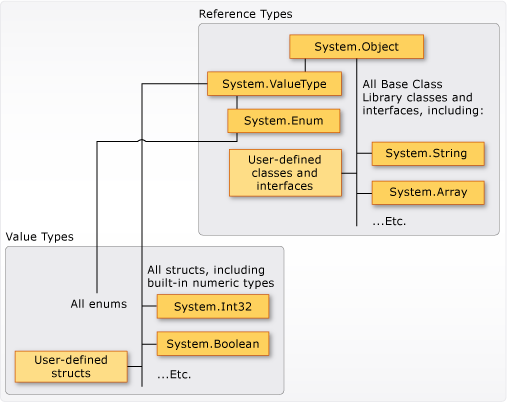
\includegraphics[width=0.78\linewidth]{img/valuetypescts.png}
	\label{fig:valuetypescts}
\end{figure}

\end{frame}

\subsection{Exemplos}
\begin{frame}[fragile]
\frametitle{Exemplo de \textit{Struct} em \CS}
\begin{lstlisting}[title=Definição da Struct Livro em \CS]
public struct Livro
{
	public string autor;
	public string titulo;
	public int anoPublicacao;
}

\end{lstlisting}
\end{frame}


\begin{frame}[fragile]
\frametitle{Exemplo de classe em \CS}
\begin{lstlisting}[title=Definição da classe Pessoa em \CS]
using System;

namespace Slides.Slide1
{
	class Pessoa
	{        
		private int idade;
		public int Idade 
		{ 
			get { return idade; } 
			set { idade = value; } 
		}
		public Sexo Sexo { get; set; }
	}
}

\end{lstlisting}
\end{frame}


\subsection{Construtores}
\begin{frame}
\frametitle{Construtores}
\begin{outline}
	\1 Sempre que uma classe ou estrutura é instanciada, o seu construtor é chamado;
	\1 Uma classe ou estrutura pode ter vários construtores que tomam diferentes argumentos;
	\1 Os Construtores permitem que o programador defina valores padrão, limitar a instanciação e escrever códigos flexíveis ao contexto e fáceis de ler.
	\1 Quando não informado, é criado um construtor padrão sem parâmetros
	\1 Um construtor é um método cujo nome é o mesmo que o nome do seu tipo;
	\1 A assinatura do método inclui apenas o nome do método e sua lista de parâmetros; 
	\2 Não inclui um tipo de retorno. 	
\1 Os construtores de instâncias são usados para criar e inicializar variáveis de membros da instância quando você usa a expressão \codef{new} para criar um objeto de uma classe.
\end{outline}
\end{frame}


\begin{frame}[fragile]
\frametitle{Exemplo construtor}
\begin{outline}
	\1 Construtor para uma classe chamada Pessoa.
\2 [Ex.:] \begin{lstlisting}
public class Pessoa
{
	private string ultimoNome;
	private string primeiroNome;
	
	public Pessoa(string primeiroNome, string ultimoNome)
	{
		this.primeiroNome = primeiroNome;
		this.ultimoNome = ultimoNome;
	}
}
\end{lstlisting}
\1 Construtor implementado com um simples comando
\2 [Ex.:] \begin{lstlisting}
	public Pessoa(string name) => primeiroNome = name;
\end{lstlisting}
\end{outline}
\end{frame}


\subsection{Modificadores de Acesso}
\begin{frame}
\frametitle{Modificadores de Acesso}
\begin{outline}
	\1 Os modificadores de acesso são palavras-chave usadas para especificar a acessibilidade declarada de um membro ou de um tipo. 
	\2 \textbf{public}: o acesso não está restrito.
	
	\2 \textbf{protected}: o acesso é limitado à classe ou tipos de conteúdo derivados da classe que contém.
	
	\2 \textbf{internal}: o acesso é limitado ao assembly corrente.
	
	\2 \textbf{protected internal}: o acesso é limitado ao assembly corrente ou tipos derivados da classe que contém.
	
	\2 \textbf{private}: o acesso é limitado ao tipo de conteúdo.
	
\end{outline}
\end{frame}






\subsection{Interfaces e Herança}

\begin{frame}[fragile]
\frametitle{Interface}
\begin{outline}
	\1 A definição de uma interface é dada pela seguinte estrutura:
	
\2 \begin{lstlisting}
interface <<NomeDaInterface>>
{
	<< Comportamentos >>
}
\end{lstlisting}
\1 Use o caractere \codef{:} (dois pontos) para indicar que uma classe/interface implementará os comportamento. Este mesmo caractere é utilizado para a herança de classes.
\end{outline}
\end{frame}


\begin{frame}[fragile]
\frametitle{Herança/Polimorfismo}
\begin{outline}
	\1 O membro derivado deve usar o modificador \codef{override} explicitamente;
	\1 Uma classe derivada somente pode substituir um membro da classe se ele foi declarado como \codef{abstract} ou \codef{virtual}.
	\1 A palavra reservada \codef{base} é equivalente ao \codef{super} do Java;
		
\end{outline}
\begin{columns}[T]
	\begin{column}{0.5\textwidth}
\begin{lstlisting}	
class SerVivo
{
	// ...
	// Campos
	// ...
	public SerVivo(int idade)
	{
		....
	}	
}
\end{lstlisting}		
	\end{column}
	\begin{column}{0.5\textwidth}	
\begin{lstlisting}
class Pessoa : SerVivo
{
	// ...
	// Campos
	// ...
	public Pessoa(): base(0){
	}
}
\end{lstlisting}
	\end{column}
\end{columns}
\end{frame}

%
%\begin{frame}[fragile]
%\frametitle{Exercício Herança}
%\begin{outline}
%	\1 Sabe-se que um \texttt{\underline{Carro}} é um \texttt{\underline{Veiculo}}
%	\1 Os \texttt{\underline{Veiculo}} andam, e cada um faz a sua maneira: carro $\neq$ avião $\neq$ trem;
%	\1 Os \texttt{\underline{carros}} conseguem virar para a direita e esquerda, já os \texttt{\underline{trens}} não;
%	\1 Os \texttt{\underline{carros}} andam para frente, trás, direita e esquerda;
%	\1 Os \texttt{\underline{Carros}} realizam a operação de \texttt{\underline{abrir}} e \texttt{\underline{fechar}}, já as \texttt{\underline{bicicletas}} não possuem esta funcionalidade;
%	\1 Um \texttt{\underline{Ser vivo}}, apesar de não ser um \texttt{\underline{Veiculo}}, consegue \texttt{\underline{andar}} para frente, trás, direita e esquerda;
%	\1 Um \texttt{\underline{Ser vivo}}, apesar de não ser um \texttt{\underline{Carro}}, consegue \texttt{\underline{abrir}} e \texttt{\underline{fechar}};	
%\end{outline}
%\end{frame}
%
%\begin{frame}[fragile]
%\frametitle{Exercício Herança com Interface}
%\begin{outline}
%	\1 [1.] O que um \texttt{\underline{notebook}}, um \texttt{\underline{Carro}} e um \texttt{\underline{cofre}} tem em comum? 
%	\2 R: Ambos realizam a operação de \texttt{\underline{abrir}} e \texttt{\underline{fechar}};
%	\1 [2.] O que um \texttt{\underline{ser vivo}} e um \texttt{\underline{carro}} tem em comum? 
%	\2 R: Ambos \texttt{\underline{andam}} para frente para trás e para a direita/esquerda.
%	\1 Diante das respostas acima, crie as classes dos objetos listados que atende as interfaces \codef{IAbrirFechar} e \codef{IMovimento} conforme definição a seguir:
%	
%\end{outline}
%\begin{columns}[T]
%	\begin{column}{0.5\textwidth}
%\begin{lstlisting}
%interface IAbirFechar{
%	void Abrir();
%	void Fechar();
%	Situacao Situacao {get;}
%	void Trancar();
%}
%\end{lstlisting}
%	\end{column}
%	\begin{column}{0.5\textwidth}	
%\begin{lstlisting}
%inteface IMovimento {
%	void Andar(int qtdMetros, Direcao direcao);
%	void Virar(int angulo);
%}
%\end{lstlisting}		
%	\end{column}
%\end{columns}
%\end{frame}


\begin{frame}[fragile]
\frametitle{Atenção}
\begin{outline}
	\1 Tanto uma classe quanto um método pode ser abstrato. 
	\1 Para isso utilize a palavra reservada \codef{abstract};
	\1 Métodos virtuais (\codef{virtual}) podem ser redefinidos através da palavra \codef{override};
	\1 Quando um método/classe é \codef{selead} não é permitida a sobrescrita dele(a).
	\1 Para criar constantes use a palavra reservada \codef{const}
	\2 Quando criadas, seus valores são computados em tempo de compilação;
	\1 [] \begin{lstlisting}
internal const int IDADE_ESPERADA_NO_INICIO = 0;	
	\end{lstlisting}
	\1 Também é possível fazer com que um campo seja \codef{readonly}
	\1 [] \begin{lstlisting}
public static readonly MinhasCores Vermelho = new MinhasCores(255, 0, 0);	
	\end{lstlisting}
	\note{ver \Codigos\ifs-cbsi-programacaoweb3-2014-1\Slides\Slide1\MinhasCores.cs}
\end{outline}
\end{frame}


\begin{frame}[fragile]
\frametitle{Exercício}
\begin{outline}
	\1 Implemente um programa que é responsável por gerenciar figuras geométricas como Quadrado, Retângulo e Circulo;
		\2 O programa deverá conseguir gerenciar uma lista de até 20 figuras;
		\2 Deverá apresentar um menu para:
			\3 [1.] Manter (CRUD) uma figura;
			\3 [2.] Listar a área de figura com base no ID;
			\3 [3.] Apresentar um relatório contendo o ID|Nome|Data Criação|área ordenado pelo Nome;	
			\3 [4.] Listar a figura com maior lado.		
		\2 O \codef{quadrado} é um subtipo de \codef{Retângulo} 		
	\1 Toda figura atende a \textit{interface} \codef{IFigura} conforme especificado abaixo:
	\1 []
\begin{lstlisting}
public interface IFigura
{
	long ID {get;}
	string Nome { get; }
	double Area { get; }
	DateTime DataCriacao { get; }
}
\end{lstlisting}
\end{outline}
\end{frame}


\section{Exceções}

\begin{frame}[fragile]
\frametitle{Exceções}
\begin{outline}
	\1 O bloco \codef{try...catch.. finally} captura e executa ações adicionais para o tratamento da exceção;
	\1 A herança da classe \codef{Exception} permite personalizar a exceção;
	\1 Assim como no Java, o \codef{throw} lança um erro no programa
\1 []
\begin{lstlisting}
try 	//bloco obrigatório
{
	//código para ser executado normalmente
}
catch ( Exception erro) //Bloco opcional
{
	//interceptação do erro
	Console.WriteLine(erro.Message);
}
finally 	//Bloco opcional
{
	//executa indepente da situação (erro ou sucesso)
}
\end{lstlisting}
\end{outline}
\end{frame}

\section{Generics e Partial Classes and Methods}
\subsection{Generics}

\begin{frame}
\frametitle{Generics}
\begin{outline}
	\1 Generics apresenta o conceito de parâmetros tipados;
	\1 Tornam possível a concepção classes e métodos que adiam a especificação de um ou mais tipos até que a classe ou método seja declarado e instanciado pelo código do cliente do .NET Framework;
	\1 Seu uso maximizar reutilização de código, segurança de tipo e desempenho;
	\1 A palavra \codef{default(T)} inicializa a variável com o valor padrão para o tipo da classe;	
\end{outline}
\end{frame}


\begin{frame}[fragile]
\frametitle{Exemplo Generics}
\begin{outline}
\1 Definição Genérica
\1 [] 
\begin{lstlisting}
public class GenericList<T>
{
	void Add(T input) { }
	public int Count()
	{
		return 0;
	}
	public bool FazNada<U>(T parametro1, U parametro2)
	{
		return parametro1.Equals(parametro2);
	}
}
\end{lstlisting}
\1 Uso:
\1 []
\begin{lstlisting}
GenericList<int> list1 = new GenericList<int>();
list1.FazNada<bool>(0,false);
\end{lstlisting}
\end{outline}
\end{frame}


\begin{frame}[fragile]
\frametitle{Exercício}
\begin{outline}
	\1 Implemente uma pilha usando \codef{Generics}. As operações permitidas são:	
	\1 []
	\begin{lstlisting}
interface IPilha<T>
{
	bool IsEmpty(); 
	bool IsFull();
	T Pop(); //Exceção se estiver vazia
	void Push(T value);
}	
	\end{lstlisting}
\end{outline}
\end{frame}

\begin{frame}[fragile]
\frametitle{Teste para a implementação}
\lstinputlisting{codigos/testePilha.cs}
\end{frame}

\subsection{Partial Classes and Methods}

\begin{frame}
\frametitle{Partial Classes and Methods}
\begin{outline}
	\1 Com o .NET é possível quebrar a definição de um método, \codef{class}, \codef{struct} ou \codef{interface} em um ou mais arquivos;
	\1 Todas as partes são combinadas no momento da instanciação;
	\1 Fazer uso da palavra reservada \codef{partial};	
\end{outline}
\end{frame}


\section{Leitura complementar}
\begin{frame}
\frametitle{Leitura complementar}
\begin{outline}
	\1 \textit{Tipos de dados do \CS}		
	\2 \href{https://docs.microsoft.com/en-us/dotnet/csharp/programming-guide/types/index}{Types (\CS Programming Guide)}
	\2 \href{http://msdn.microsoft.com/en-us/library/ya5y69ds.aspx}{Built-In Types Table (\CS Reference)}
	\1 Propriedades 
	\2 \href{https://docs.microsoft.com/en-us/dotnet/csharp/programming-guide/classes-and-structs/properties}{Trabalhando com propriedades}
	\2 \href{https://docs.microsoft.com/en-us/dotnet/csharp/programming-guide/indexers/comparison-between-properties-and-indexers}{Comparison Between Properties and Indexers (\CS Programming Guide)}
	\1 Construtores e Instâncias
	\2 \href{https://docs.microsoft.com/en-us/dotnet/csharp/programming-guide/classes-and-structs/using-constructors}{ Using Constructors }
	\2 \href{https://docs.microsoft.com/en-us/dotnet/csharp/programming-guide/classes-and-structs/instance-constructors}{Instance Constructors}
	\1 Operadores
	\2 \href{https://docs.microsoft.com/en-us/dotnet/csharp/programming-guide/statements-expressions-operators/operators}{Operators}
	\1 \href{https://docs.microsoft.com/en-us/dotnet/csharp/programming-guide/inside-a-program/coding-conventions}{\CS Coding Conventions}
	\1 \href{https://docs.microsoft.com/en-us/dotnet/csharp/language-reference/keywords/access-modifiers}{Modificadores de acesso}
	\1 \href{https://docs.microsoft.com/en-us/dotnet/csharp/language-reference/keywords/switch}{Case/Switch}
\end{outline}
\end{frame}
\end{document}